%%%%%%%%%%%%%%%%%%%%%%%%%%%%%%%%%%%%%%%%%%%%%%%%%%%%%%%%%%%%%%%%%%%%%%%%
% Plantilla TFG/TFM
% Escuela Politécnica Superior de la Universidad de Alicante
% Realizado por: Jose Manuel Requena Plens
% Contacto: info@jmrplens.com / Telegram:@jmrplens
%%%%%%%%%%%%%%%%%%%%%%%%%%%%%%%%%%%%%%%%%%%%%%%%%%%%%%%%%%%%%%%%%%%%%%%%

\chapter{Resultados}
\label{resultados}

\section{Evaluación y Pruebas de Concepto}
\label{sec:evaluacion}

Para validar la viabilidad de los componentes clave del sistema LLMSearch, especialmente en lo referente a la búsqueda semántica y la gestión de embeddings, se realizaron pruebas de concepto utilizando la base de datos vectorial ChromaDB. Esta sección detalla un experimento específico diseñado para ilustrar cómo ChromaDB maneja la creación, almacenamiento, búsqueda y visualización de embeddings a partir de un conjunto de documentos de ejemplo.

El objetivo principal de esta prueba fue observar la capacidad de ChromaDB para:
\begin{itemize}
    \item Generar representaciones vectoriales (embeddings) de fragmentos de texto.
    \item Almacenar estos embeddings de forma persistente.
    \item Realizar búsquedas semánticas basadas en la similitud del coseno entre el embedding de una consulta y los embeddings de los documentos almacenados.
    \item Facilitar la comprensión de las relaciones semánticas mediante herramientas de visualización.
\end{itemize}

\subsection{Configuración del Experimento con ChromaDB}
Se utilizó un script de Python que interactúa con una instancia local y persistente de ChromaDB. \textbf{El código completo de este script de prueba se puede encontrar en el Anexo \ref{anx:chroma_script}.} Se definió un corpus de ocho documentos de texto concisos, cuyos temas giran en torno a la programación (Python), los embeddings, las bases de datos vectoriales (ChromaDB) y el procesamiento del lenguaje natural. Los documentos empleados fueron:
\begin{enumerate}
    \item \textit{"Python is a high-level, interpreted programming language"}
    \item \textit{"Embeddings are vector representations of text"}
    \item \textit{"Chroma is a vector database for storing embeddings"}
    \item \textit{"Language models can generate semantic embeddings"}
    \item \textit{"3D visualization helps to understand the distance between embeddings"}
    \item \textit{"Vector databases are useful for semantic searches"}
    \item \textit{"Embeddings capture the semantics of words and phrases"}
    \item \textit{"Python has many libraries for natural language processing"}
\end{enumerate}
Estos documentos fueron procesados para generar sus respectivos embeddings utilizando el modelo de embedding por defecto de ChromaDB. Posteriormente, se creó una colección denominada \texttt{"example\_embeddings"} donde se almacenaron los documentos junto con sus embeddings.

\subsection{Resultados de la Búsqueda Semántica}
Se realizó una búsqueda semántica utilizando la consulta: \texttt{"What are embeddings?"}. El sistema fue instruido para devolver los 3 resultados más similares. Los resultados obtenidos, incluyendo el documento y su distancia semántica respecto a la consulta, se muestran en la Figura \ref{fig:chroma_console_eval}.

\begin{figure}[H]
\centering
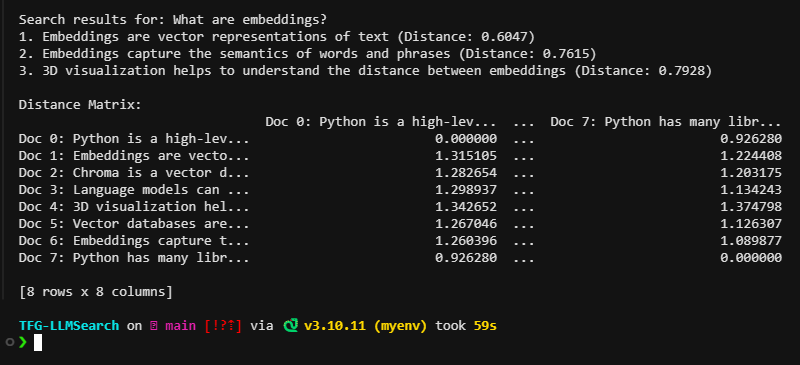
\includegraphics[width=0.8\textwidth]{archivos/chroma_console.png}
\caption[Resultados de Búsqueda Semántica en Consola con ChromaDB]{Salida de consola mostrando los resultados de la búsqueda para la consulta "¿What are embeddings?". Se observa que los documentos más relevantes, con menor distancia, son recuperados.}
\label{fig:chroma_console_eval}
\end{figure}

Como se aprecia en la Figura \ref{fig:chroma_console_eval}, los documentos recuperados son altamente pertinentes a la consulta. El documento \textit{"Embeddings are vector representations of text"} es el más cercano (menor distancia), seguido por \textit{"Embeddings capture the semantics of words and phrases"} y \textit{"Language models can generate semantic embeddings"}. Esto demuestra la capacidad de ChromaDB para identificar y priorizar documentos semánticamente relevantes a una consulta en lenguaje natural.

\subsection{Visualización de Embeddings}

Para comprender mejor la distribución espacial y las relaciones semánticas entre los documentos y la consulta, se generaron dos tipos de visualizaciones.

\subsubsection{Visualización 3D de Embeddings}
Los embeddings de los ocho documentos y el embedding de la consulta fueron proyectados en un espacio tridimensional utilizando técnicas de reducción de dimensionalidad (como PCA o t-SNE, aplicadas internamente por la utilidad de visualización de ChromaDB). El resultado se muestra en la Figura \ref{fig:chroma_3d_eval}.

\begin{figure}[H]
\centering
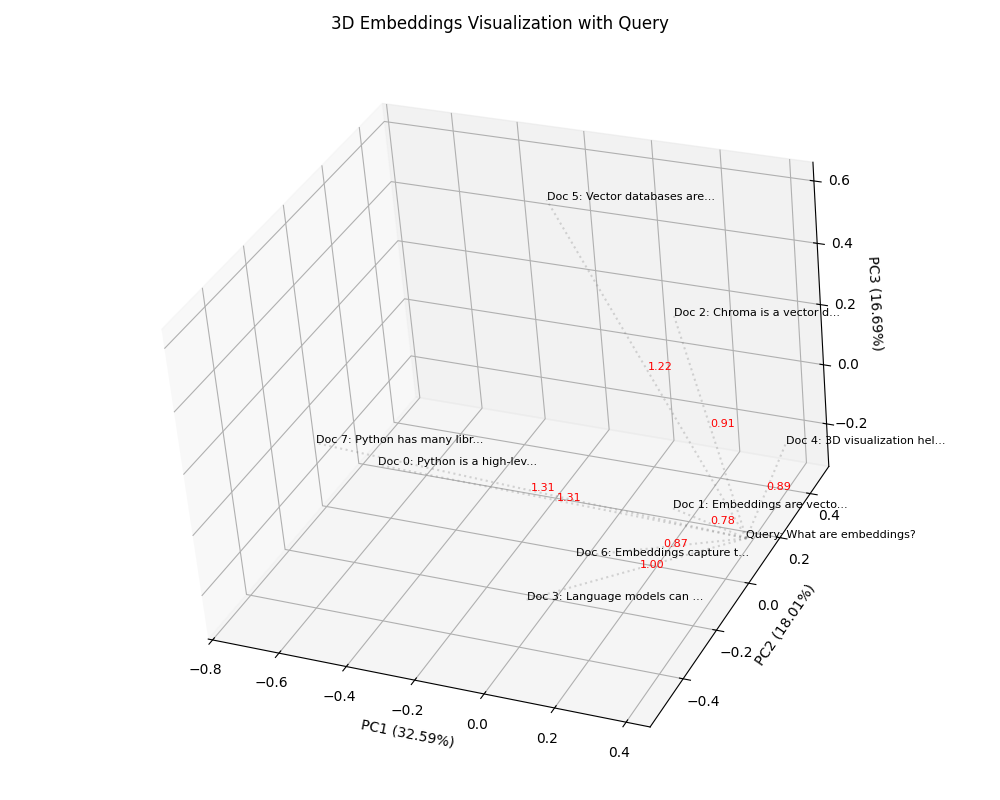
\includegraphics[width=\textwidth]{archivos/chroma_3d.png}
\caption[Visualización 3D de Embeddings con ChromaDB]{Representación 3D de los embeddings de los documentos de ejemplo y la consulta. El punto de la consulta ("Query: What are embeddings?") está resaltado.}
\label{fig:chroma_3d_eval}
\end{figure}

En la Figura \ref{fig:chroma_3d_eval}, cada punto representa un embedding. Se puede observar cómo los documentos semánticamente similares tienden a agruparse. El punto correspondiente a la consulta \texttt{"Query: What are embeddings?"} se encuentra espacialmente cercano a los embeddings de los documentos que tratan sobre embeddings (por ejemplo, "Doc 1: Embeddings are...", "Doc 6: Embeddings capt..."). Esta proximidad visual corrobora los resultados numéricos de la búsqueda.

\subsubsection{Matriz de Distancias Semánticas}
Para obtener una visión cuantitativa de las distancias entre todos los pares de documentos, se generó una matriz de distancias. Esta matriz (Figura \ref{fig:chroma_dist_matrix_eval}) muestra la distancia semántica (por ejemplo, distancia coseno) entre cada par de embeddings de los documentos originales.

\begin{figure}[H]
\centering
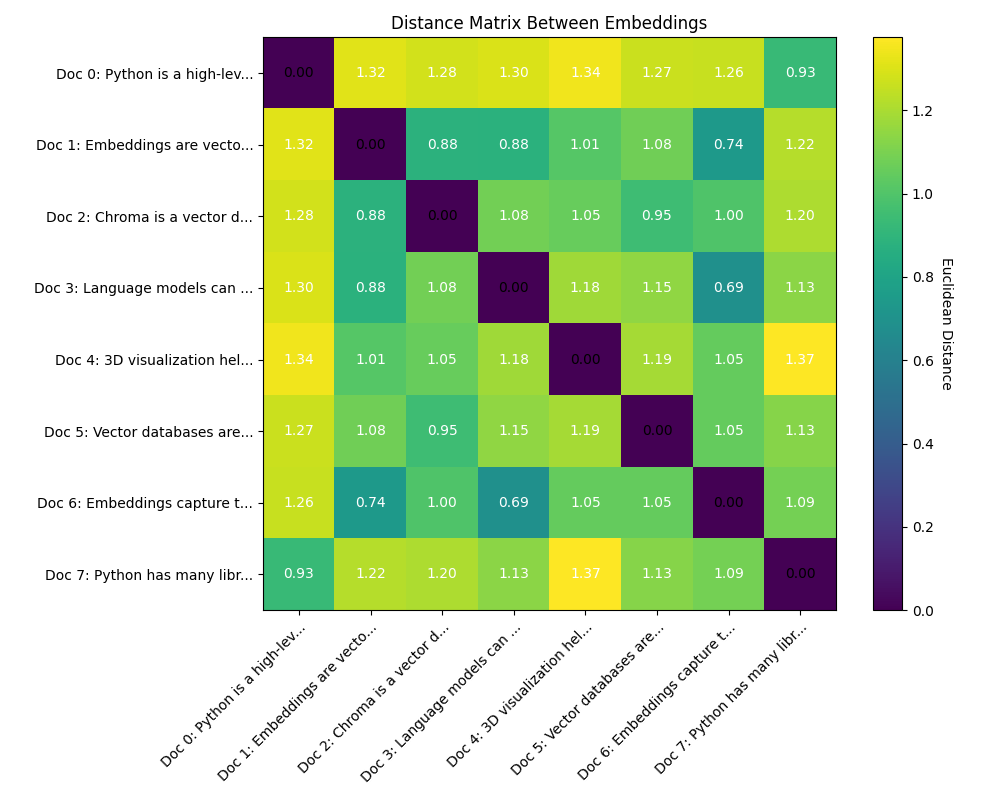
\includegraphics[width=0.9\textwidth]{archivos/chroma_confussion_matrix.png} % Asegúrate que esta imagen sea realmente una matriz de distancias
\caption[Matriz de Distancias Semánticas entre Documentos con ChromaDB]{Matriz de distancias que muestra la similitud semántica par a par entre los documentos de ejemplo. Colores más oscuros indican menor distancia (mayor similitud).}
\label{fig:chroma_dist_matrix_eval}
\end{figure}

La Figura \ref{fig:chroma_dist_matrix_eval} (asumiendo que la imagen `chroma\_confussion\_matrix.png` es en realidad una matriz de distancias como la generada por `visualize\_matriz\_distances`) permite identificar clústeres de documentos semánticamente relacionados. Por ejemplo, los documentos que hablan sobre "Python" podrían mostrar distancias menores entre sí en comparación con documentos que hablan exclusivamente sobre "embeddings".

\subsection{Conclusiones de la Evaluación Preliminar}
Las pruebas realizadas con ChromaDB demuestran su idoneidad como componente central para la funcionalidad de búsqueda semántica en LLMSearch. La capacidad de generar, almacenar y buscar embeddings eficientemente, junto con las herramientas para visualizar y comprender las relaciones semánticas, son fundamentales para el proyecto.

Esta evaluación preliminar valida la elección de una base de datos vectorial como ChromaDB. Pruebas de rendimiento más exhaustivas con volúmenes de datos mayores y diferentes tipos de ficheros serán necesarias en etapas posteriores para evaluar la escalabilidad y optimizar la configuración del sistema. Sin embargo, esta prueba de concepto inicial es prometedora y sienta una base sólida para el desarrollo de las capacidades de búsqueda inteligente de LLMSearch.